\section{Обзор существующих моделей}
\label{sec:Chapter2} \index{Chapter2}

\subsection{Модели для распознавания ключевых точек на теле человека}

В данном разделе мы рассмотрим 5-6 (УТОЧНИТЬ ПОСЛЕ ОПИСАНИЯ) различных моделей. В \autoref{sec:Chapter4} мы выберем 4 наиболее удобные в использовании и в обучении и проведем эксперимент по оценке данных моделей.

Так же хочется сказать, что, помимо приведенных, есть множество моделей от одиночных авторов, не объединенных в лаборатории \cite{pet_recognition, pet_classification}. Они в основном брали какую-то из представленных ниже моделей и проводили небольшое улучшение.

А теперь перейдем к моделям.

\subsubsection{BlazePose}

MediaPipe является одним из проектов компании GOOGLE и в своей работе решает задачи компьютерного зрения. В нем уже были представлены модели для распознавания лица (Face Detection) и его поверхности (Face Mesh), ладоней (Hands), объектов (Object Detection и Objectron) и другие \cite{mediapipe}. Для нас же интересна задача поиска ключевых точек, которую и решает модель BlazePose \cite{BlazePose}. На момент исследования модель умеет отслеживать движения человека на видеофрагменте и строить покадровую маску человека.

Для предложенной модели была создана топология, которая представляет собой суперпозицию топологии COCO и двух других топологий, уже использовавшихся в других подпроектах MediaPipe. Об этом более подробно написано в \autoref{subsec:Theory of keypoint detection}.

\hfill \break
В BlazePose используется top-down подход оценки позы человека. Сначала запускается Pose Detector (см \autoref{fig:mp_model_structure}), который возвращает координаты интересующей нас области (region-of-interest или ROI). Алгоритм используем расширение модели BlazeFace для определения наличия человека в кадре. Поэтому данная модель чувствительна к видимости головы, лица в частности, на фотографии. Взяв идею витрувианского человека Леонардо Да Винчи, исследователям понадобилось ещё две точки для точной локализации человека на изображении.

\begin{figure}[h]
	\centering
	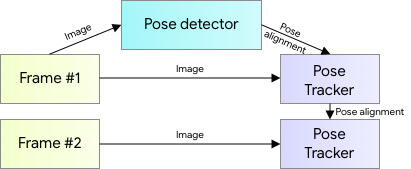
\includegraphics[width=\textwidth * 4 / 5]{./images/MPPose/Model_structure.jpg}
	\caption{Структура модели BlazePose для работы в реальном времени.\\ \href{https://1.bp.blogspot.com/-J66lTDBjlgw/XzVwzgeQJ7I/AAAAAAAAGYM/WBIhbOqzi4ICUswEOHv8r7ItJIOJgL9iwCLcBGAsYHQ/s411/image11.jpg}{Оригинальное изображение}}
	\label{fig:mp_model_structure}
\end{figure}

Следующим шагом Pose Tracker производит локализацию каждой точки в заданной ROI. Данное действие производится путем комбинированной обработки тепловой карты и данных о смещении с использованием регрессионной модели (см \autoref{fig:mp_architecture}). (ВОЗМОЖНО СТОИТ ПОЧИТАТЬ ПРО ТАКУЮ ОБРАБОТКУ И ПОПОДРОБНЕЕ ЕЕ ОПИСАТЬ)

\begin{figure}[h]
	\centering
	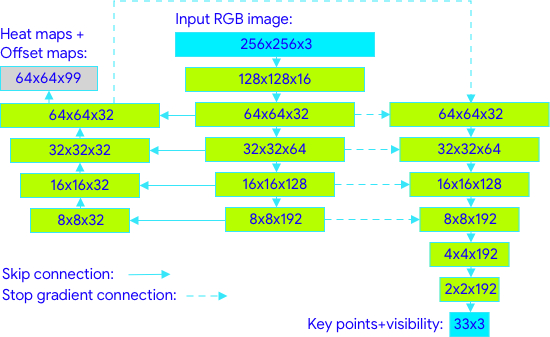
\includegraphics[width=\textwidth * 4 / 5]{./images/MPPose/architecture.jpg}
	\caption{Архитектура модели Pose Tracker.\\ \href{https://1.bp.blogspot.com/-XxKesnBALGM/XzVxSKZNWZI/AAAAAAAAGYc/WOt31icjp_YyjMxz06RSEwTi9K3qviFxwCLcBGAsYHQ/s550/image9.jpg}{Оригинальное изображение}}
	\label{fig:mp_architecture}
\end{figure}

Как можно заметить из \autoref{fig:mp_model_structure}, при аналитике видеофрагмента Pose Detector используется только на первом кадре, ведь позже данные об интересующей нас области передаются от кадра к кадру. Это упрощает вычисления и позволяет ускорить работу модели в реальном времени.

Развитием данной моели есть ее полное объединение с моделями BlazeFace и BlazeHand в модель Holistic \cite{Holistic}. Она рассматривает намного большее количество точек на лице и ладонях. 




\subsubsection{MoveNet.SinglePose}

SinglePose создана для работы в веб-интерфейсах или на мобильных устройствах в режиме реального времени. Модель представлена в двух спецификациях: lightning и thunder. Первая является менее требовательной в плане мощностей и вычислений и способна обрабатывать до 50 кадров в секунду. В то же время, по заверениям создателей, вторая модель имеет большие запросы по ресурсам, но дает лучшую точность распознавания, правда со скоростью до 30 кадров в секунду.

За расположение ключевых точек выбрана классическая топология COCO. Поэтому возвращает модель координаты 17 точек, которые нормированы на размер изображения (лежат в отрезке [0, 1]).

\hfill \break
Представленная модель реализована на архитектуре MobileNetV2 \cite{mobilenetv2}. (СЛОЖНАЯ АРХИТЕКТУРА. НЕОБХОДИМО ПРО НЕЕ ПРОЧИТАТЬ, А ПОТОМ УЖЕ ДОПИСАТЬ ДАННЫЙ РАЗДЕЛ.)

Также существует развитие проекта MoveNet в MoveNet.MultiPose для распознавания сразу нескольких людей на изображении. Усовершенствованная модель также представлена в двух вариациях. В данной работе много персональное распознавание позы не исследовалось.




\subsubsection{OpenPose}

OpenPose (OP) - это подпроект CMU-Perceptual-Computing-Lab из университета Карнеги-Меллона. В нем представлены различные модели: от локализации точного положения кистей и лица, до определения позы, исследуя 135 точек на теле человека. Также ОР может распознавать нескольких человек одновременно и поддерживает отслеживание скелета человека на видеозаписи в реальном времени через веб-камеру.

В текущей работе рассмотрим модель, работающую по топологии из 25 точек - чем-то похожую на топологию Halpe (см. \autoref{subsec:Theory of keypoint detection}). Особенностью является определение положения стоп за счет детекции 3 дополнительных точек на каждой из них.

OpenPose тоже использует сверточные нейронные сети для решении задачи распознавания ключевых точек с помощью bottom-up подхода. В своей работе исследователи используют понятия карты достоверности обнаружения точки, карты двумерных векторных полей ориентации конечностей (Part Affinity Fields или PAFs) и графы соответствия обнаруженных точек определенным людям на изображении.

Первым шагом происходит обработка изображения и построение карт достоверности и PAFs, про которое поговорим позже. Вторым шагов происходит сопоставление точек и конечностей отдельным людям с использованием графов соответствия. Они помогают решить данную задачу и быстрее решать задачу построения скелетов нескольких человек. В итоге на выходе мы имеем скелеты нескольких человек. Все шаги представлены на \autoref{fig:op_structure}.

\begin{figure}[h]
	\centering
	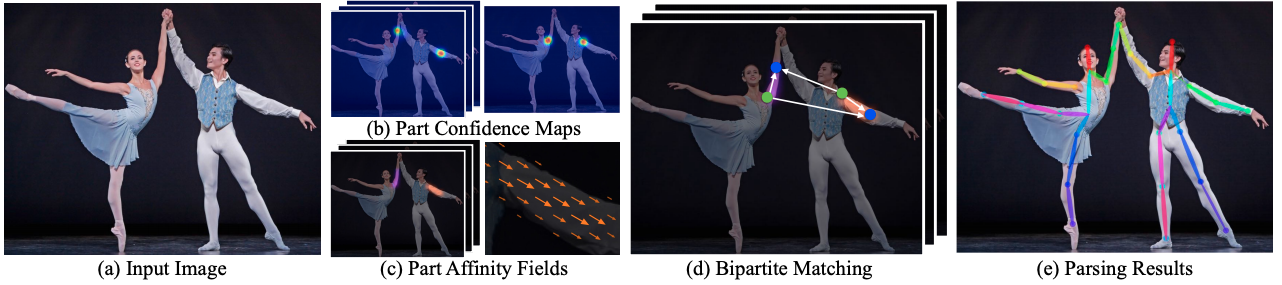
\includegraphics[width=\textwidth]{./images/OpenPose/structure}
	\caption{Последовательность распознавания ключевых точек моделью OpenPose.\\ \href{https://miro.medium.com/0*rXablSR1mU2Mn-cG.png}{Оригинальное изображение}}
	\label{fig:op_structure}
\end{figure}

В первоначальной версии модели \cite{OpenPose_first} вычисление карт достоверности и PAFs происходило параллельно, в два этапа. Но в последней работе \cite{OpenPose} предсказания поставили последовательно, так как из PAFs интуитивно можно предсказать и уточнить карты достоверности обнаружения точки (см. \autoref{fig:op_architecture}). Ещё были заменены ядра свертки размером 7х7 на блоки из 3-х последовательных ядер 3х3 (см. \autoref{fig:op_architecture}). Эти преобразование помогло почти в 200 раз увеличить скорость распознавания и в 7 раз улучшить точность.

\begin{figure}[h]
	\centering
	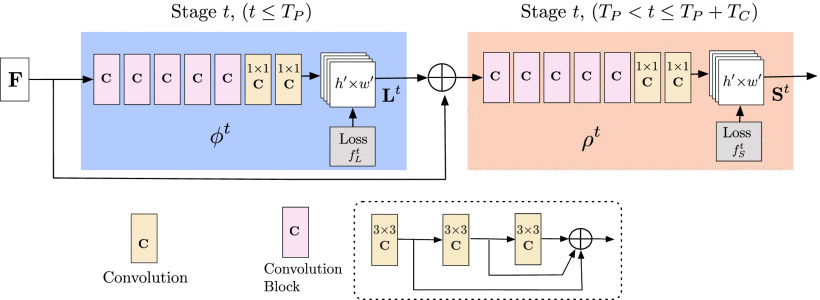
\includegraphics[width=\textwidth * 4 / 5]{./images/OpenPose/architecture.jpg}
	\caption{Архитектура модели OpenPose 2D Pose Estimation.\\ \href{https://ieeexplore.ieee.org/mediastore_new/IEEE/content/media/34/9280439/8765346/cao3-2929257-large.gif}{Оригинальное изображение}}
	\label{fig:op_architecture}
\end{figure}




\subsubsection{MMPose}

MMPose - является подпроектом лаборатории Open-MMLab \cite{mmpose2020}. Изначально проект рассматривал решение задачи детектирования объектов, но позже развивались подпроекты, связанные с компьютерным зрением. Изначально был проект MMSkeleton, основанный на исследовании ST-GCN \cite{STGCN}. Позже появился проект MMPose, включающий в себя распознавание ключевых точек и восстановление скелета человека, модель Animal для тех же задач, но на теле животных. Причем задачи, связанные с человеком, имеют решения с получением предсказаний в 2-х мерном и в 3-х мерном вариантах.

Данная модель постоянно улучшается и подключает новые мировые достижения в свои работы. MMPose использует top-down подход в своей работе и другие наработки лаборатории Open-MMLab. Для работы необходимо сначала использовать detection model, а потом уже передать данные о локализованных людях в pose model.

Детектор натренирован на датасете COCO и выдает предсказания в соответствии с его 17 точечной топологией. Также есть скрипты для обучения на других наборах данных, за что спасибо разработчикам. Правда эти наборы данных надо сначала скачать, но об этом в \autoref{sec:Chapter4}.




\subsubsection{AlphaPose}

AlphaPose является основной наработкой проекта Machine Vision and Intelligence Group из Шанхайского университета транспорта (Shanghai Jiao Tong University или SJTU). Это первая модель, которая получила значение метрики mAP на датасете COCO выше 70 (0.7) и выше 80 на MPII. Поддерживается как на Linux, так и на Windows. Обрабатывает видео и поддерживает слежение за человеком в реальном времени через восстановление его скелета.

Исследователи не против объединяться с другими проектами для улучшения качества модели и проработки новый фичей. Одной из таких коопераций стала топология Halpe (см. \autoref{subsec:Theory of keypoint detection}), на основании которой и производится оценка позы человека. Доступными являются варианты также с 17 точками от COCO и 25 и 135 точек от Halpe.

В работе Alpha использует top-down подход. Первым этапом идет Faster R-CNN для детектирования человека и выдачи прямоугольников. После используется модель RMPE для предсказания различных поз, которые может принимать  человек. Последним этапом идет работа p-Pose NMS для устранению избыточных предсказаний. На выходе мы получаем изображение с восстановленными позами людей. Все шаги представлены на \autoref{fig:ap_structure}. \cite{fang2017rmpe}

\begin{figure}[h]
	\centering
	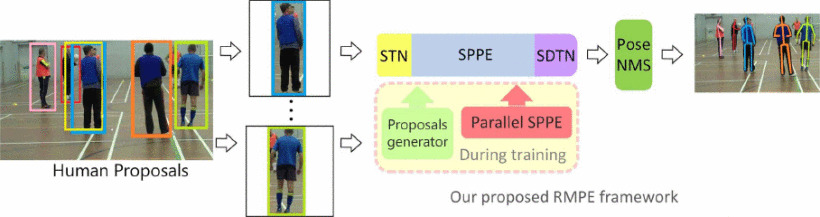
\includegraphics[width=\textwidth]{./images/AlphaPose_structure}
	\caption{Пример работы сети AlphaPose.\\ \href{https://ieeexplore.ieee.org/mediastore_new/IEEE/content/media/8234942/8237262/8237518/8237518-fig-3-source-large.gif}{Оригинальное изображение}}
	\label{fig:ap_structure}
\end{figure}

Рассмотрим поближе модель предсказания. Она использует симметричное преобразование spatial transformer network (STN) и обратное ему spatial de-transformer network (SDTN). Они введены для исправления ошибок локализации, так как SPPE, представленная между ними (см. \autoref{fig:ap_architecture}), является очень чувствительной к неточностям прямоугольника. При обучении параллельно основной модели добавляется ещё одна SPPE (см. \autoref{fig:ap_architecture}) для корректировки преобразования STN. Таким образом мы приблизим данные, получаемые предсказателем, к идеальным и получим наиболее точный результат.

\begin{figure}[h]
	\centering
	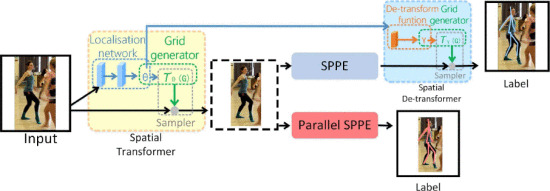
\includegraphics[width=\textwidth]{./images/AlphaPose_architecture}
	\caption{Архитектура сети RMPE.\\ \href{https://ieeexplore.ieee.org/mediastore_new/IEEE/content/media/8234942/8237262/8237518/8237518-fig-4-source-small.gif}{Оригинальное изображение}}
	\label{fig:ap_architecture}
\end{figure}




\subsubsection{DeepPose}

DeepPose является одним из самых первых решений задачи распознавания ключевых точек на теле человека с помощью глубокого обучения. Статья "DeepPose: Human Pose Estimation via Deep Neural Networks"{} \cite{DeepPose} была представлена исследователями из GOOGLE на конференции CVPR в 2014 году.

В своей работе они представили каскад из DNN-регрессоров для локализации суставов тела. На тот момент принятых топологий ещё не было и поза кодировалась координатами суставов, нормализованными на размер изображения.
Первым этапом применялась CNN для локализации точки, а вторым каскадом применялись DNN для уточнения результата (см. \autoref{fig:dp_architecture}). Таким образом получалось довольно точно распознавать ключевые точки на фотографии.

\begin{figure}[h]
	\centering
	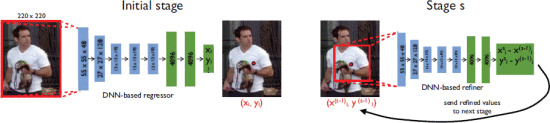
\includegraphics[width=\textwidth]{./images/DeepPose}
	\caption{Архитектура сети DeepPose.\\ \href{https://ieeexplore.ieee.org/mediastore_new/IEEE/content/media/6909096/6909393/6909610/6909610-fig-2-source-small.gif}{Оригинальное изображение}}
	\label{fig:dp_architecture}
\end{figure}





\subsection{Модели для классификации позы человека}

В данном разделе мы рассмотрим 3 различных модели, которые можно использовать для классификации движений человека. 

\subsubsection{MMaction2 by OpenMMlab}

Что-то сложное от китайцев.

\subsubsection{BlazePose by MediaPipe}

Просто накинули сверху предыдущей модели kNN.

\subsubsection{mmakos}

Чувак взял OpenPose и добавил классификатор.


\newpage